% Copyright 2021  Ed Bueler

\documentclass[xcolor={svgnames},
               hyperref={colorlinks,citecolor=DeepPink4,linkcolor=FireBrick,urlcolor=Maroon}]
               {beamer}

\mode<presentation>{
  \usetheme{Madrid}
  \usecolortheme{seagull}
  \setbeamercovered{transparent}
  \setbeamerfont{frametitle}{size=\large}
}

\setbeamercolor*{block title}{bg=red!10}
\setbeamercolor*{block body}{bg=red!5}

\usepackage[english]{babel}
\usepackage[latin1]{inputenc}
\usepackage{times}
\usepackage[T1]{fontenc}
% Or whatever. Note that the encoding and the font should match. If T1
% does not look nice, try deleting the line with the fontenc.

\usepackage{empheq,bm}
\usepackage{xspace}
\usepackage{verbatim,fancyvrb}

\usepackage{tikz}
\usetikzlibrary{shapes,arrows.meta,decorations.markings,decorations.pathreplacing,fadings,positioning}

\usepackage[kw]{pseudo}
\pseudoset{left-margin=15mm,topsep=5mm,idfont=\texttt,st-left=,st-right=}


% If you wish to uncover everything in a step-wise fashion, uncomment
% the following command:
%\beamerdefaultoverlayspecification{<+->}

\newcommand{\ba}{\mathbf{a}}
\newcommand{\bb}{\mathbf{b}}
\newcommand{\bc}{\mathbf{c}}
\newcommand{\bbf}{\mathbf{f}}
\newcommand{\bg}{\mathbf{g}}
\newcommand{\bn}{\mathbf{n}}
\newcommand{\bq}{\mathbf{q}}
\newcommand{\br}{\mathbf{r}}
\newcommand{\bx}{\mathbf{x}}
\newcommand{\by}{\mathbf{y}}
\newcommand{\bv}{\mathbf{v}}
\newcommand{\bu}{\mathbf{u}}
\newcommand{\bw}{\mathbf{w}}

\newcommand{\bF}{\mathbf{F}}
\newcommand{\bG}{\mathbf{G}}
\newcommand{\bQ}{\mathbf{Q}}

\newcommand{\grad}{\nabla}
\newcommand{\Div}{\nabla\cdot}
\newcommand{\minmod}{\operatorname{minmod}}

\newcommand{\CC}{\mathbb{C}}
\newcommand{\RR}{\mathbb{R}}

\newcommand{\ddt}[1]{\ensuremath{\frac{\partial #1}{\partial t}}}
\newcommand{\ddx}[1]{\ensuremath{\frac{\partial #1}{\partial x}}}
\newcommand{\Matlab}{\textsc{Matlab}\xspace}
\newcommand{\Octave}{\textsc{Octave}\xspace}
\newcommand{\eps}{\epsilon}

\newcommand{\ip}[2]{\left<#1,#2\right>}

\newcommand{\xiphalf}{{x_{i+\frac{1}{2}}}}
\newcommand{\ximhalf}{{x_{i-\frac{1}{2}}}}
\newcommand{\Fiphalf}{{F_{i+\frac{1}{2}}}}
\newcommand{\Fimhalf}{{F_{i-\frac{1}{2}}}}
\newcommand{\Fiphalfn}{{F^n_{i+\frac{1}{2}}}}
\newcommand{\Fimhalfn}{{F^n_{i-\frac{1}{2}}}}

\newcommand{\trefcolumn}[1]{\begin{bmatrix} \phantom{x} \\ #1 \\ \phantom{x} \end{bmatrix}}
\newcommand{\trefmatrixtwo}[2]{\left[\begin{array}{c|c|c} & & \\ #1 & \dots & #2 \\ & & \end{array}\right]}
\newcommand{\trefmatrixthree}[3]{\left[\begin{array}{c|c|c|c} & & & \\ #1 & #2 & \dots & #3 \\ & & & \end{array}\right]}
\newcommand{\trefmatrixgroups}[4]{\left[\begin{array}{c|c|c|c|c|c} & & & & & \\ #1 & \dots & #2 & #3 & \dots & #4 \\ & & & & & \end{array}\right]}

\newcommand{\blocktwo}[4]{\left[\begin{array}{c|c} #1 & #2 \\ \hline #3 & #4 \end{array}\right]}

\newcommand{\bqed}{{\color{blue}\qed}}
\newcommand{\ds}{\displaystyle}

\newcommand\mynum[1]{{\renewcommand{\insertenumlabel}{#1}%
      \usebeamertemplate{enumerate item} \,}}


\title{Getting started on machine learning}

\subtitle{{with one little artificial neural net}}

\author{Ed Bueler}

\institute[UAF]{MATH 692 Mathematics for Machine Learning \\ UAF}

\date[Spring 2022]{13 January 2022}

%\titlegraphic{\begin{picture}(0,0)
%    \put(0,180){\makebox(0,0)[rt]{\includegraphics[width=4cm]{figs/software.png}}}
%  \end{picture}
%}

%% this nonsense needed to start section counter at 0; see
%% https://tex.stackexchange.com/questions/170222/change-the-numbering-in-beamers-table-of-content
\makeatletter
\patchcmd{\beamer@sectionintoc}
  {\ifnum\beamer@tempcount>0}
  {\ifnum\beamer@tempcount>-1}
  {}
  {}
%\beamer@tocsectionnumber=-1
\makeatother


\begin{document}
\beamertemplatenavigationsymbolsempty

\begin{frame}
  \maketitle
\end{frame}

\begin{frame}{today's talk}

\begin{itemize}
\item \alert{my topic:} {\small how this $\downarrow$ neural network does this $\downarrow$ classification task}

\medskip
\hspace{5mm} 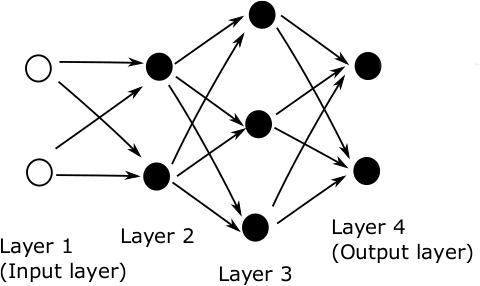
\includegraphics[height=30mm]{figs/network.png} \hfill 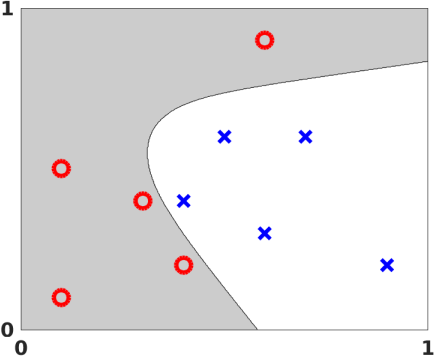
\includegraphics[height=30mm]{figs/classification} \hspace{10mm}

\bigskip
\item an \alert{example} from this $\downarrow$ paper:

\medskip

HH19 \, $=$ \, 
\begin{minipage}[t]{0.75\textwidth} \footnotesize
C.~F.~Higham \& D.~J.~Higham (2019). \href{http://www.math.stonybrook.edu/~bishop/classes/math533.S21/MachineLearning/SIAMreview.pdf}{\emph{Deep learning: An introduction for applied mathematicians.}} SIAM Review, 61(4), 860-891
\end{minipage}
\end{itemize}
\end{frame}


\begin{frame}{today's talk}

\begin{itemize}
\item \alert{goal for today.} know the meanings of ML language:

\medskip
\small
\qquad \begin{tabular}{ll}
\emph{artificial neuron} \qquad & \emph{activation function} \\
\emph{weight matrix} & \emph{bias vector} \\
\emph{training} & \emph{stochastic gradient descent} \\
\emph{back-propagation}
\end{tabular}

\medskip
\item ML = machine learning
\item which standard mathematical concept(s) match these buzzwords?
\end{itemize}
\end{frame}


\begin{frame}{big caveat}

\begin{itemize}
\item I am no expert on what I am talking about here
\item many in room know more than me
\item I volunteered to give one intro talk, that's all!
\end{itemize}
\end{frame}


\begin{frame}{\emph{participant}-driven seminar logistics}

\begin{itemize}
\item sign-up sheet!
\item my existing webpages:
    \begin{itemize}
    \item[$\circ$] \href{http://bueler.github.io/M692S22/index.html}{\texttt{bueler.github.io/M692S22}}
    \item[$\circ$] \href{https://github.com/bueler/ml-seminar}{\texttt{github.com/bueler/ml-seminar}}
    \end{itemize}
\item in-person or hybrid?
    \begin{itemize}
    \item[$\circ$] is this classroom adequate?
    \end{itemize}
\item what will be the topics?
    \begin{itemize}
    \item[$\circ$] are there out-of-bounds topics?
    \item[$\circ$] who is volunteering to talk?
    \end{itemize}
\end{itemize}
\end{frame}


\begin{frame}{Outline}
  \tableofcontents[hideallsubsections]
\end{frame}

\section{a single artificial neuron}

\begin{frame}{artificial neuron $=$ nonlinear-ized inner product}

\begin{columns}
\begin{column}{0.55\textwidth}
\begin{itemize}
\item given (column) vectors $v,{\color{blue} w} \in \RR^n$
\item recall \emph{inner product}:
    $$\ip{{\color{blue} w}}{v} = {\color{blue} w}^\top v = \sum_{j=1}^n {\color{blue} w_j} v_j$$
\item apply a nonlinear function $\sigma: \RR^1 \to \RR^1$:
\only<1>{
\begin{equation*}
{\color{red} a} = \sigma\left(\sum_{j=1}^n {\color{blue} w_j} v_j\right) \in \RR^1
\end{equation*}
}
\only<2>{
\begin{equation*}
{\color{red} a} = \sigma\left(\sum_{j=1}^n {\color{blue} w_j} v_j + {\color{ForestGreen} b}\right) \in \RR^1
\end{equation*}
}
    \begin{itemize}
    \item<2>[$\circ$] detail: add a bias ${\color{ForestGreen} b} \in \RR^1$
    \item<2>[$\circ$] that's it! an \alert{artificial neuron}
    \end{itemize}
\end{itemize}
\end{column}
\begin{column}{0.45\textwidth}
\only<1>{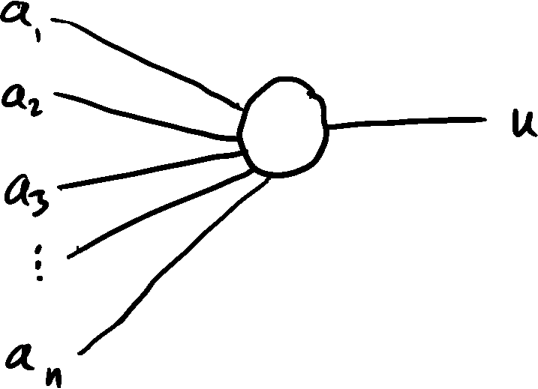
\includegraphics[width=\textwidth]{figs/single-neuron}}
\only<2>{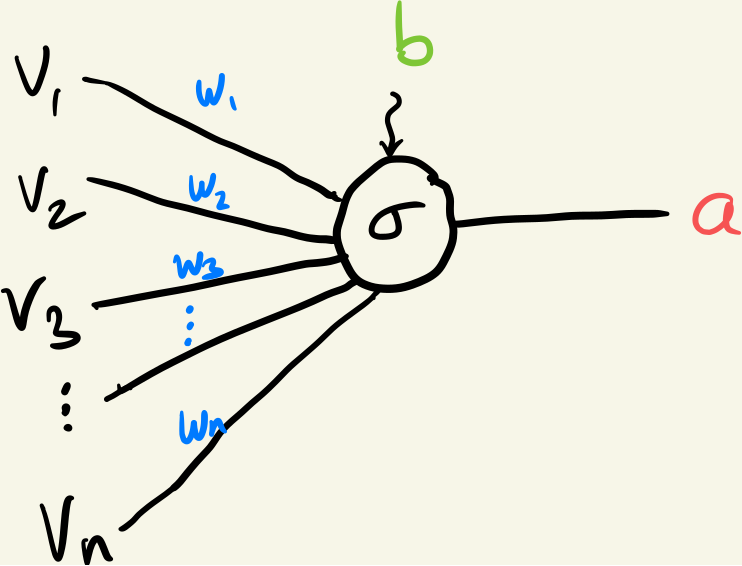
\includegraphics[width=\textwidth]{figs/b-single-neuron}}
\end{column}
\end{columns}
\end{frame}


\begin{frame}{neuron roles}

\begin{columns}
\begin{column}{0.55\textwidth}
\begin{itemize}
\item $v$ is input
\item \alert{weights} ${\color{blue} w}$ and \alert{biases} ${\color{ForestGreen} b}$ are parameters
    \begin{itemize}
    \item[$\circ$] they need \alert{training}
    \end{itemize}
\item the \alert{activation function} $\sigma$ is fixed
\item the output ${\color{red} a}$ is the \alert{activation} of the neuron
\end{itemize}
\end{column}
\begin{column}{0.45\textwidth}
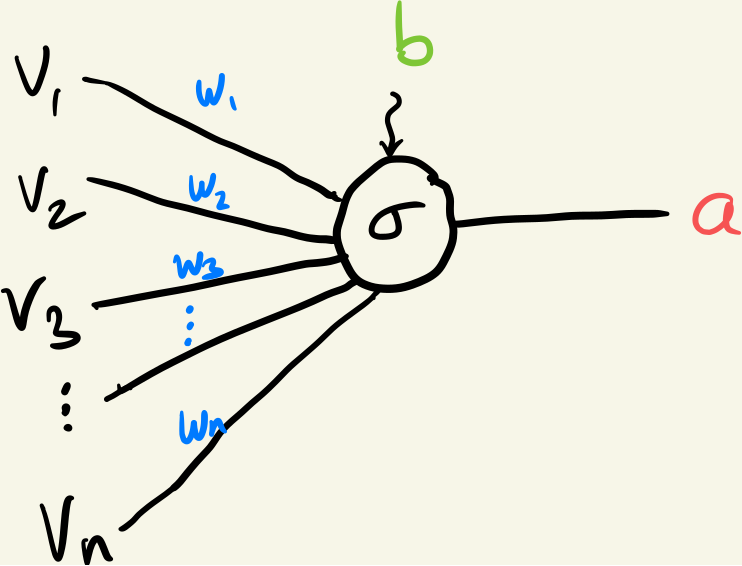
\includegraphics[width=\textwidth]{figs/b-single-neuron}

\begin{equation*}
{\color{red} a} = \sigma\left(\sum_{j=1}^n {\color{blue} w_j} v_j + {\color{ForestGreen} b}\right)
\end{equation*}
\end{column}
\end{columns}
\end{frame}


\begin{frame}{nonlinear activation function}

\begin{center}
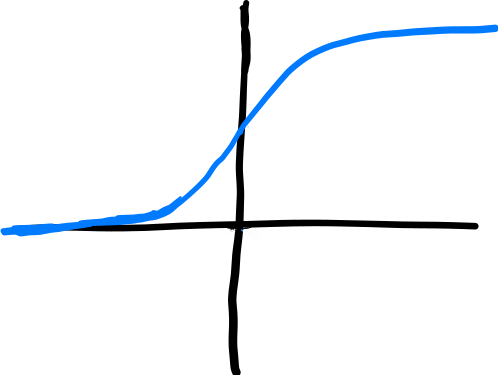
\includegraphics[height=30mm]{figs/sigmoid} \hspace{10mm} 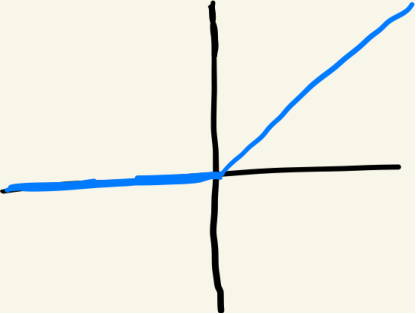
\includegraphics[height=30mm]{figs/relu}

sigmoid \hspace{42mm} ReLU \phantom{fo}
\end{center}

\begin{itemize}
\item $\sigma$ is the \alert{activation function}
    \begin{itemize}
    \item[$\circ$] an increasing scalar function with bounded derivative
    \end{itemize}
\item some possibilities:
    \begin{itemize}
    \item[$\circ$] \alert{sigmoid}, e.g.\qquad $\displaystyle \sigma(z) = \frac{1}{1 + e^{-z}}$
    \item[$\circ$] \alert{rectified linear unit (ReLU)},\qquad $\displaystyle \sigma(z) = \begin{cases} z, & z > 0 \\ 0, & z \le 0 \end{cases}$
    \end{itemize}
\end{itemize}
\end{frame}


\begin{frame}{a trained neuron}

\begin{columns}
\begin{column}{0.6\textwidth}
\begin{itemize}
\item a \alert{trained neuron} is one with known parameters ${\color{blue} w},{\color{ForestGreen} b}$
\item then ${\color{red} a}:\RR^n \to \RR^1$ is a known function:
    $${\color{red} a} = {\color{red} a}(v)$$

    \begin{itemize}
    \item[$\circ$] similar cost to inner product
    \item[$\circ$] backward stable
    \item[$\circ$] one might write ${\color{red} a}(v;{\color{blue} w},{\color{ForestGreen} b})$ to make dependence on parameters clear
    \end{itemize}
\end{itemize}
\end{column}
\begin{column}{0.4\textwidth}
\hfill 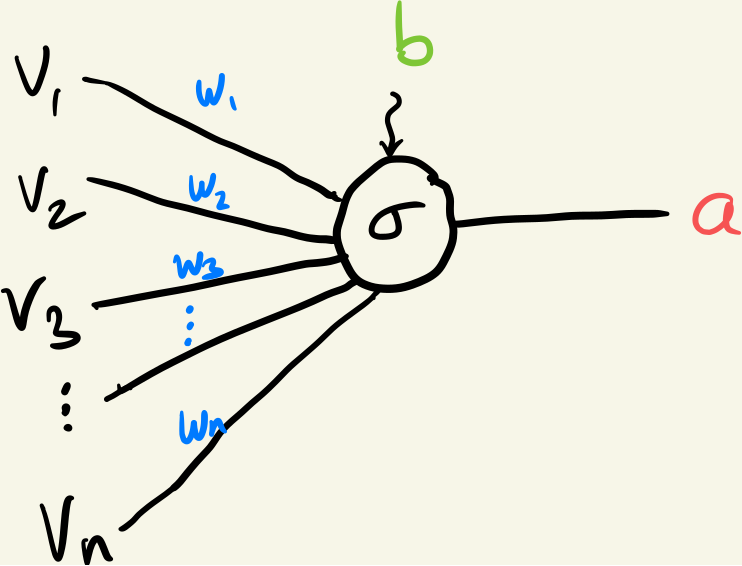
\includegraphics[width=0.9\textwidth]{figs/b-single-neuron}
\end{column}
\end{columns}
\end{frame}


\section{forward through a neural net}

\begin{frame}{Outline}
  \tableofcontents[hideallsubsections,currentsection]
\end{frame}


\begin{frame}{feed-forward networks}

\begin{center}
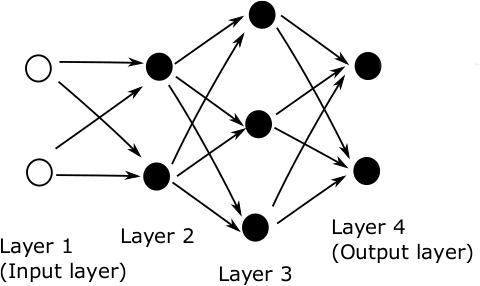
\includegraphics[height=30mm]{figs/network}
\end{center}

\begin{itemize}
\item considering only \alert{feed-forward} networks
    \begin{itemize}
    \item[$\circ$] edges connect consecutive layers, in order
    \item[$\circ$] in ML language: feed-forward versus \alert{recurrent}
    \item[$\circ$] in graph language: ``feed-forward network'' $=$ connected, directed acyclic graph which is equal to its own transitive reduction
    \end{itemize}
\end{itemize}
\end{frame}


\begin{frame}{network notation}

\begin{center}
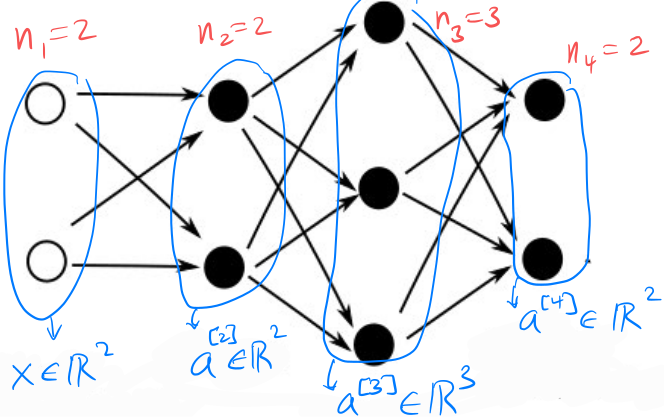
\includegraphics[height=35mm]{figs/state-notation}
\end{center}

\begin{itemize}
\item notation from HH19
\item ${\color{red} n_\ell}$ is number of neurons in layer $\ell=1,\dots,L$
    \begin{itemize}
    \item[$\circ$] $\ell=1$ is \alert{input} layer
    \item[$\circ$] input values are first-layer activations: $x = {\color{blue} a^{[1]}} \in \RR^{{\color{red} n_1}}$
    \item[$\circ$] $\ell=L$ is \alert{output} layer
    \item[$\circ$] output values are final-layer activations: $y = {\color{blue} a^{[L]}} \in \RR^{{\color{red} n_L}}$
    \end{itemize}
\item activations in layer $\ell$ form a vector ${\color{blue} a^{[\ell]}} \in \RR^{{\color{red} n_\ell}}$
    \begin{itemize}
    \item[$\circ$] ${\color{blue} a_j^{[\ell]}}$ is activation of neuron $j$ in layer $\ell$
    \end{itemize}
\end{itemize}
\end{frame}


\begin{frame}{weight notation}

\begin{center}
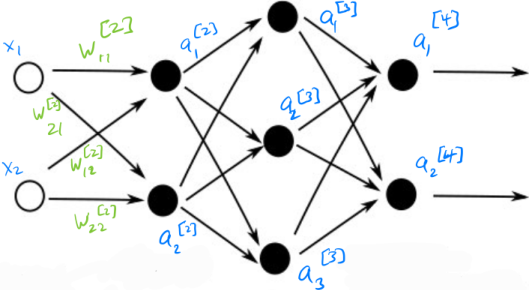
\includegraphics[height=40mm]{figs/weight-notation}
\end{center}

\begin{itemize}
\item weight ${ \color{ForestGreen} w_{jk}^{[\ell]} }$ on the edge from neuron ${\color{blue} a_k^{[\ell-1]}}$ to neuron ${\color{blue} a_j^{[\ell]}}$
\item thus
    $${\color{blue} a_j^{[\ell]}} = \sigma\left(\sum_{k=1}^{n_{\ell-1}} {\color{ForestGreen} w_{jk}^{[\ell]}} {\color{blue} a_k^{[\ell-1]}} + b_j\right)$$
\item which suggests matrix-vector multiplication!
\end{itemize}
\end{frame}


\begin{frame}{weight notation using vectors and matrices}

\begin{center}
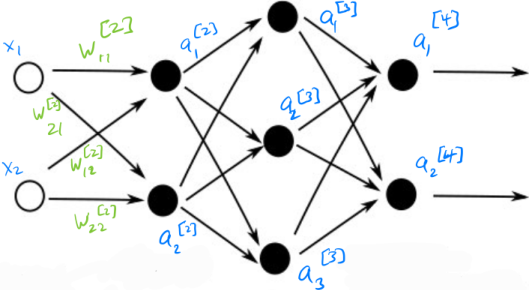
\includegraphics[height=25mm]{figs/weight-notation}
\end{center}

\begin{itemize}
\item one (row) vector of weights for each neuron
\item the inputs to the neurons in a layer are weighted by a matrix:
    $${\color{ForestGreen} W^{[\ell]}} = \left(\text{weights into layer $\ell$}\right) = \begin{bmatrix} {\color{ForestGreen} w_{jk}^{[\ell]}} \end{bmatrix}$$

    \begin{itemize}
    \item[$\circ$] ${\color{ForestGreen} W^{[\ell]}}$ is $n_{\ell}\times n_{\ell-1}$
    \end{itemize}
\item assuming $\sigma$ applied entrywise:
    $${\color{blue} a^{[\ell]}} = \sigma\left({\color{ForestGreen} W^{[\ell]}} {\color{blue} a^{[\ell-1]}} + b^{[\ell]}\right)$$

    \begin{itemize}
    \item[$\circ$] also: bias vector $b^{[\ell]} \in \RR^{n_{\ell}}$
    \end{itemize}
\end{itemize}
\end{frame}


\begin{frame}{forward pass = nonlinear-ized matrix multiplication}

\begin{center}
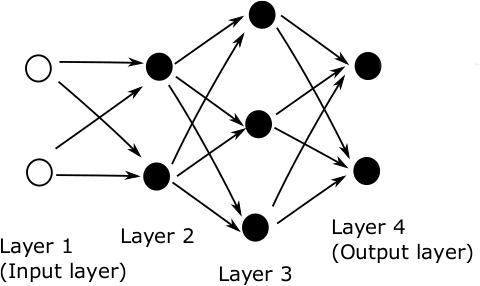
\includegraphics[height=25mm]{figs/network}
\end{center}

\begin{itemize}
\item for this small $L=4$ network:
\begin{align*}
y = a^{[4]} &= \sigma\left(W^{[4]} a^{[3]} + b^{[4]}\right) = \dots \\
            &= \sigma\left(W^{[4]} \sigma\left(W^{[3]} \sigma\left(W^{[2]} a^{[1]} + b^{[2]}\right) + b^{[3]}\right) + b^{[4]}\right) \\
            &= \sigma\left(W^{[4]} \sigma\left(W^{[3]} \sigma\left(W^{[2]} x + b^{[2]}\right) + b^{[3]}\right) + b^{[4]}\right)
\end{align*}
\item \emph{simplified:} if $\sigma(z)=z$ and $b^{[\ell]}=0$ then $y = W^{[4]} W^{[3]} W^{[2]} x$
\item feed-forward network = nonlinear- \& affine-ized matrix product
\end{itemize}
\end{frame}


\begin{frame}{forward-pass neural network formulas}

\begin{itemize}
\item compute from input $x = a^{[1]}$ to output $y = a^{[L]}$ by layers:
    $$a^{[\ell]} = \sigma\left(W^{[\ell]} a^{[\ell-1]} + b^{[\ell]}\right) \qquad \text{for } \ell=2,3,\dots,L$$

    \begin{itemize}
    \item[$\circ$] equation (3.2) in HH19
    \end{itemize}
\item a forward pass is an obvious loop:

\begin{pseudo*}
\pr{forward}(x)\text{:} \\+
    $a^{[1]} = x$ \\
    for $\ell = 2,3,\dots,L$: \\+
        $z^{[\ell]} = W^{[\ell]} a^{[\ell-1]} + b^{[\ell]}$ \\
        $a^{[\ell]} = \sigma\left(z^{[\ell]}\right)$ \\-
    return $y=a^{[L]}$
\end{pseudo*}

    \begin{itemize}
    \item[$\circ$] $\{W^{[\ell]}\}$ and $\{b^{[\ell]}\}$ are stored in some data structure
    \item[$\circ$] $\sigma(z)$ is implemented entrywise
    \end{itemize}
\end{itemize}
\end{frame}


\begin{frame}{forward-pass computation work model (\emph{minor point})}

\begin{itemize}
\item \alert{work} $=$ number of floating-point operations
\item work at layer $\ell$:
    $$2 n^{[\ell-1]} n^{[\ell]} + O(n^{[\ell]}) = O(n^{[\ell-1]} n^{[\ell]})$$

    \begin{itemize}
    \item[$\circ$] using big-O in the ``$n \to \infty$'' limit of big layers
    \item[$\circ$] evaluating activation functions is cheap
    \item[$\circ$] the work at one layer is basically just a matrix-vector product
    \end{itemize}
\item let $n_{\text{max}} =\max\{n^{[\ell]}\}$, the maximum layer size
\item the total forward-pass work in an $L$-layer network is asymptotically the same as $L$ matrix-vector products:
    $$\sum_{\ell=2}^L O(n^{[\ell-1]} n^{[\ell]}) = O(L n_{\text{max}}^{\,2})$$
\item \emph{note:} a forward pass is easily computed by GPU hardware
    \begin{itemize}
    \item[$\circ$] versus solving linear systems \dots
    \end{itemize}
\end{itemize}
\end{frame}


\section{training is optimization}

\begin{frame}{Outline}
  \tableofcontents[hideallsubsections,currentsection]
\end{frame}


\begin{frame}{training is a biologically-motivated procedure}

\begin{itemize}
\item imagine teaching your dog to read numbers 1,2,3:
\begin{center}
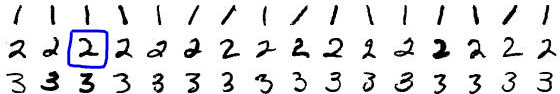
\includegraphics[width=0.7\textwidth]{figs/onetwothree}
\end{center}
\item example training procedure:
    \begin{enumerate}
    \item randomly present one image of a digit from above
\begin{center}
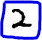
\includegraphics[width=0.1\textwidth]{figs/two} \phantom{dlasbj sadkf adsk}
\end{center}
    \item if dog barks correct number of times then gets treat

\vspace{5mm}
\hspace{10mm} \emph{bark! bark!} \qquad $\implies$

\vspace{-6mm}
\hfill 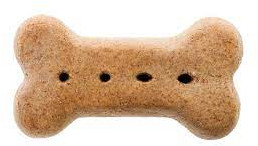
\includegraphics[width=0.15\textwidth]{figs/dogtreat} \hspace{25mm} \phantom{boo}
    \item otherwise move on to next image
    \end{enumerate}
\end{itemize}
\end{frame}


\begin{frame}{training yields persistant changes to brain}

\begin{itemize}
\item biological learning can last from hours to decades
\item something permanent/persistent changes within the brain
    \begin{itemize}
    \item[$\circ$] but neuron excitation is electrical (activation is temporary),
    \item[$\circ$] and neuron count is relatively fixed
    \end{itemize}
\item training yields chemical or morpological changes in connections between neurons, especially the \alert{synapses} where the axon connects to another neuron's dendrite
\end{itemize}

\begin{center}
\mbox{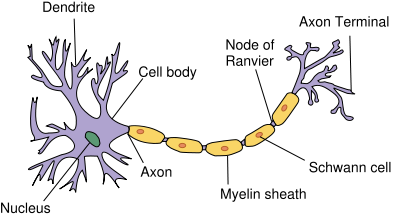
\includegraphics[width=0.5\textwidth]{figs/physicalneuron} 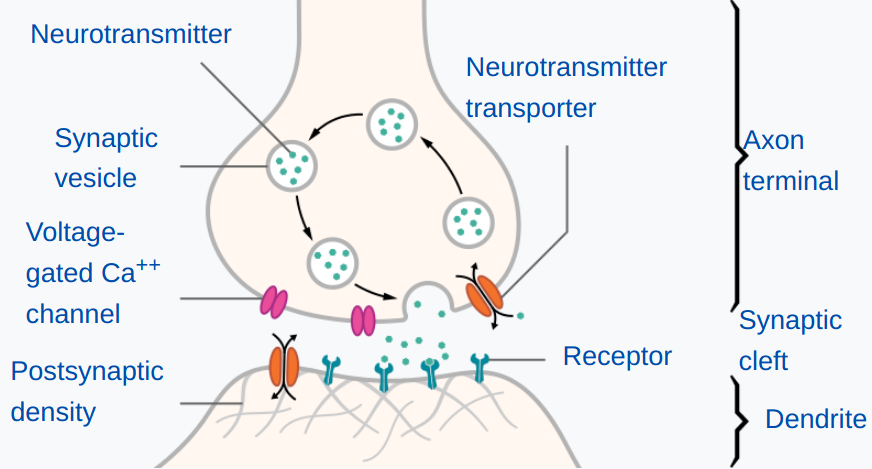
\includegraphics[width=0.4\textwidth]{figs/synapse}}
\end{center}
\end{frame}


\begin{frame}{artificial neurons as a model of real neurons}

\begin{itemize}
\item but biological realism is \emph{not} needed for machine learning!
\item we use a simplified artificial neuron:

\begin{center}
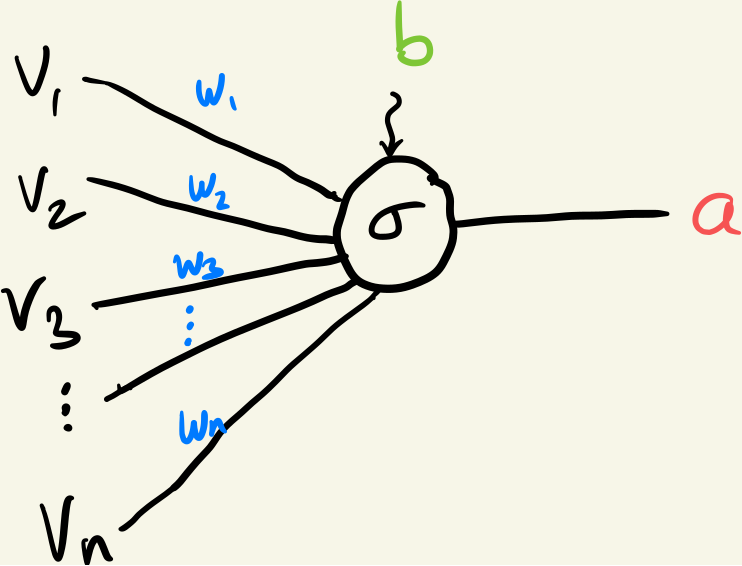
\includegraphics[width=0.3\textwidth]{figs/b-single-neuron}
\end{center}

    \begin{itemize}
    \item[$\circ$] this model is merely a formula: \quad $\displaystyle {\color{red} a} = \sigma\left(\sum_{k=1}^{n} {\color{blue} w_{k}} v_k + {\color{ForestGreen} b}\right)$
    \end{itemize}
\item however, training needs to make ``permanent'' changes in the weights ${\color{blue} w_k}$ and biases ${\color{ForestGreen} b}$
\item after training, forward passes are the network's ``learned behavior''
\end{itemize}
\end{frame}


\begin{frame}{how does training work?}

\begin{itemize}
\item so, how does training work in artificial neural networks?
\item only considering \alert{supervised training} here
\item given: $N$ pieces of \alert{labeled data} (pairs)
    $$(x^{\{i\}}, y^{\{i\}}) \qquad \text{for } i=1,\dots,N$$

    \begin{itemize}
    \item[$\circ$] $x^{\{i\}} \in \RR^{n_1}$ are the \alert{data}
    \item[$\circ$] $y^{\{i\}} \in \RR^{n_L}$ are the \alert{labels}
    \item[$\circ$] in a \alert{classification task}, the $y^{\{i\}}$ only take on finitely-many values
    \end{itemize}
\item observation: the labeled data determine the number of neurons in the first and last layers
\end{itemize}
\end{frame}


\begin{frame}{example (classification task)}

\begin{itemize}
\item example \alert{classification task} data $(x^{\{i\}},y^{\{i\}})$ in one figure

\begin{center}
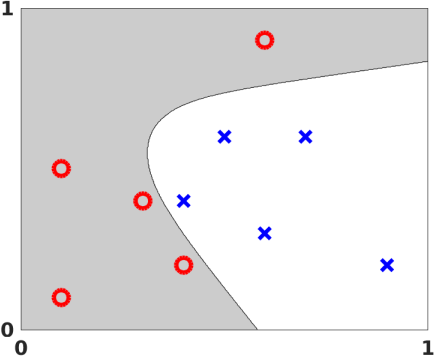
\includegraphics[height=30mm]{figs/classification}
\end{center}
    \begin{itemize}
    \item[$\circ$] $N=10$
    \item[$\circ$] marker coordinates give $x^{\{i\}} \in [0,1]^2$
    \item[$\circ$] marker type gives $y^{\{i\}}$:
   $$\text{\Large {\color{red} $\bm{\circ}$}}:\, y^{\{i\}} = \begin{bmatrix} 1 \\ 0 \end{bmatrix}, \qquad {\color{blue} \bm{\times}}:\, y^{\{i\}} = \begin{bmatrix} 0 \\ 1 \end{bmatrix} \phantom{ldsfj adflkj sadfkj adfsk}$$
    \item[$\circ$] a neural net for this data must have $n_1=n_L=2$:
    \item[$\circ$] ignore shading for now \dots
    \end{itemize}

\vspace{-15mm}
\hfill 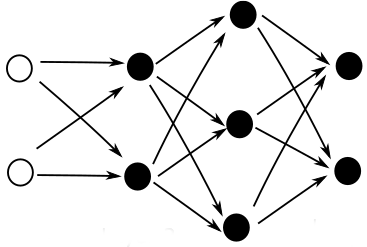
\includegraphics[width=0.2\textwidth]{figs/cleannet}
\end{itemize}
\end{frame}


\begin{frame}{a supervised training cost functional}

\begin{itemize}
\item \alert{supervised training} means choosing the weights $W^{[\ell]}$ and biases $b^{[\ell]}$, in \emph{all} the layers, so as to approximately minimize the \alert{average misfit} between the the network output from input data vector $x^{\{i\}}$ and the corresponding label vector $y^{\{i\}}$
\item using the squared $2$-norm for the misfit, this is a formula:
    $$\text{Cost} = \frac{1}{N} \sum_{i=1}^N \frac{1}{2} \|y^{\{i\}} - a^{[L]}(x^{\{i\}})\|_2^2$$

    \begin{itemize}
    \item[$\circ$] $a^{[L]}(x^{\{i\}}) =$ output-layer activation from forward pass with input $x^{\{i\}}$
    \item[$\circ$] the Cost is a scalar-valued function (\alert{functional}) of the weights and biases
    \end{itemize}
\end{itemize}
\end{frame}


\begin{frame}{better training notation}

\begin{itemize}
\item let's give all the parameters a single-letter name:
   $$p = \{W^{[2]},W^{[3]},\dots,W^{[L]},b^{[2]},b^{[3]},\dots,b^{[L]}\} \in \RR^s$$

    \begin{itemize}
    \item[$\circ$] $p$ collects all weight matrices and biases into one big column vector
    \end{itemize}
\item define the cost (misfit) of the network for one data pair:
    $$C^{\{i\}}(p) = \frac{1}{2} \left\|y^{\{i\}} - a^{[L]}(x^{\{i\}}; p)\right\|_2^2$$
\item key idea:

\medskip
\begin{quote}
The output from a forward pass through the network, namely $a^{[L]}(x^{\{i\}}; p)$, depends \emph{both} on the input data $x^{\{i\}}$ and all the weights and biases $p$.  We emphasize that the cost of one data pair is a function of $p$: $C^{\{i\}}(p)$.
\end{quote}
\end{itemize}
\end{frame}


\begin{frame}{cost functional = objective = average misfit}

\begin{itemize}
\item now define a total \alert{cost functional}, or \alert{objective}, $C(p)$
\item $C(p)$ is the \alert{average} misfit over all the labeled data:
\begin{align*}
C(p) &= \frac{1}{N} \sum_{i=1}^N C^{\{i\}}(p) \\
     &= \frac{1}{2N} \sum_{i=1}^N \left\|y^{\{i\}} - a^{[L]}(x^{\{i\}}; p)\right\|_2^2
\end{align*}
\end{itemize}
\end{frame}


\begin{frame}{training $=$ nonlinear least-squares optimization}

\begin{itemize}
\item compare
    $$C(p) = \frac{1}{2N} \sum_{i=1}^N \left\|y^{\{i\}} - a^{[L]}(x^{\{i\}}; p)\right\|_2^2$$
to ``nonlinear least-squares'' in a standard optimization textbook (Nocedal \& Wright, 2006; Chapter 10):

\medskip
\quad 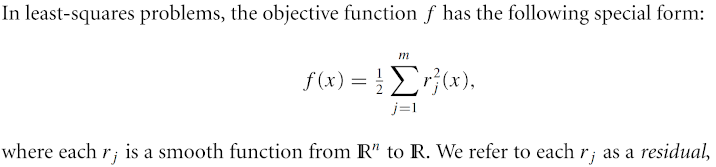
\includegraphics[width=0.8\textwidth]{figs/nls}

\medskip
\item training a neural net is \alert{nonlinear least-squares optimization}
    \begin{itemize}
    \item[$\circ$] $\left\|y^{\{i\}} - a^{[L]}(x^{\{i\}}; p)\right\|_2$ is the \alert{residual norm} for $i$th data
    \item[$\circ$] it becomes zero when the network fully-learns the $i$th data
    \end{itemize}
\end{itemize}
\end{frame}


\begin{frame}{fundamental idea: cost is a function of weights and biases}

\begin{itemize}
\item recall $p = \{W^{[2]},W^{[3]},\dots,W^{[L]},b^{[2]},b^{[3]},\dots,b^{[L]}\}$
\item the \alert{cost} for one data pair \alert{is a function of} $p$:
    $$C^{\{i\}}(p) = \frac{1}{2} \left\|y^{\{i\}} - a^{[L]}(x^{\{i\}}; p)\right\|_2^2$$
\item that is, given parameters $p$, one forward pass through the network, using input $x^{\{i\}}$, is needed to evaluate $C^{\{i\}}(p)$
\item from now on we simplify notation: \quad $\displaystyle a^{[L]} = a^{[L]}(x^{\{i\}}; p)$

\bigskip\bigskip
\item<2>[\textbf{Q.}] why is $C(p) = \frac{1}{2N} \sum_{i=1}^N \left\|y^{\{i\}} - a^{[L]}\right\|_2^2$ a function of $p$?
\item<2>[\textbf{a.}] because the activations of the final layer, namely $a^{[L]}$, are determined by the weights and biases in the network
\end{itemize}
\end{frame}


\begin{frame}{gradient descent}

\begin{itemize}
\item our goal is to minimize \quad \small $\displaystyle C(p) = \frac{1}{2N} \sum_{i=1}^N \left\|y^{\{i\}} - a^{[L]}\right\|_2^2$ \normalsize
\item the function $C(p)$ is differentiable
    \begin{itemize}
    \item[$\circ$] \emph{why? what does this assume about the network?}
    \end{itemize}
\item \dots thus we can compute the \alert{gradient} $\grad C(p)$
\item the gradient points \emph{up hill} on the surface $C:\RR^s\to\RR$,
\item natural idea: do \alert{gradient descent}
\end{itemize}

\medskip
\hspace{5mm} \mbox{\begin{pseudo*}
\pr{gd}(p)\text{:} \\+
    for $s = 1,2,\dots$: \\+
        $p \gets p - \eta \grad C(p)$ \\-
    return $p$
\end{pseudo*}}

\vspace{-20mm}
\hfill 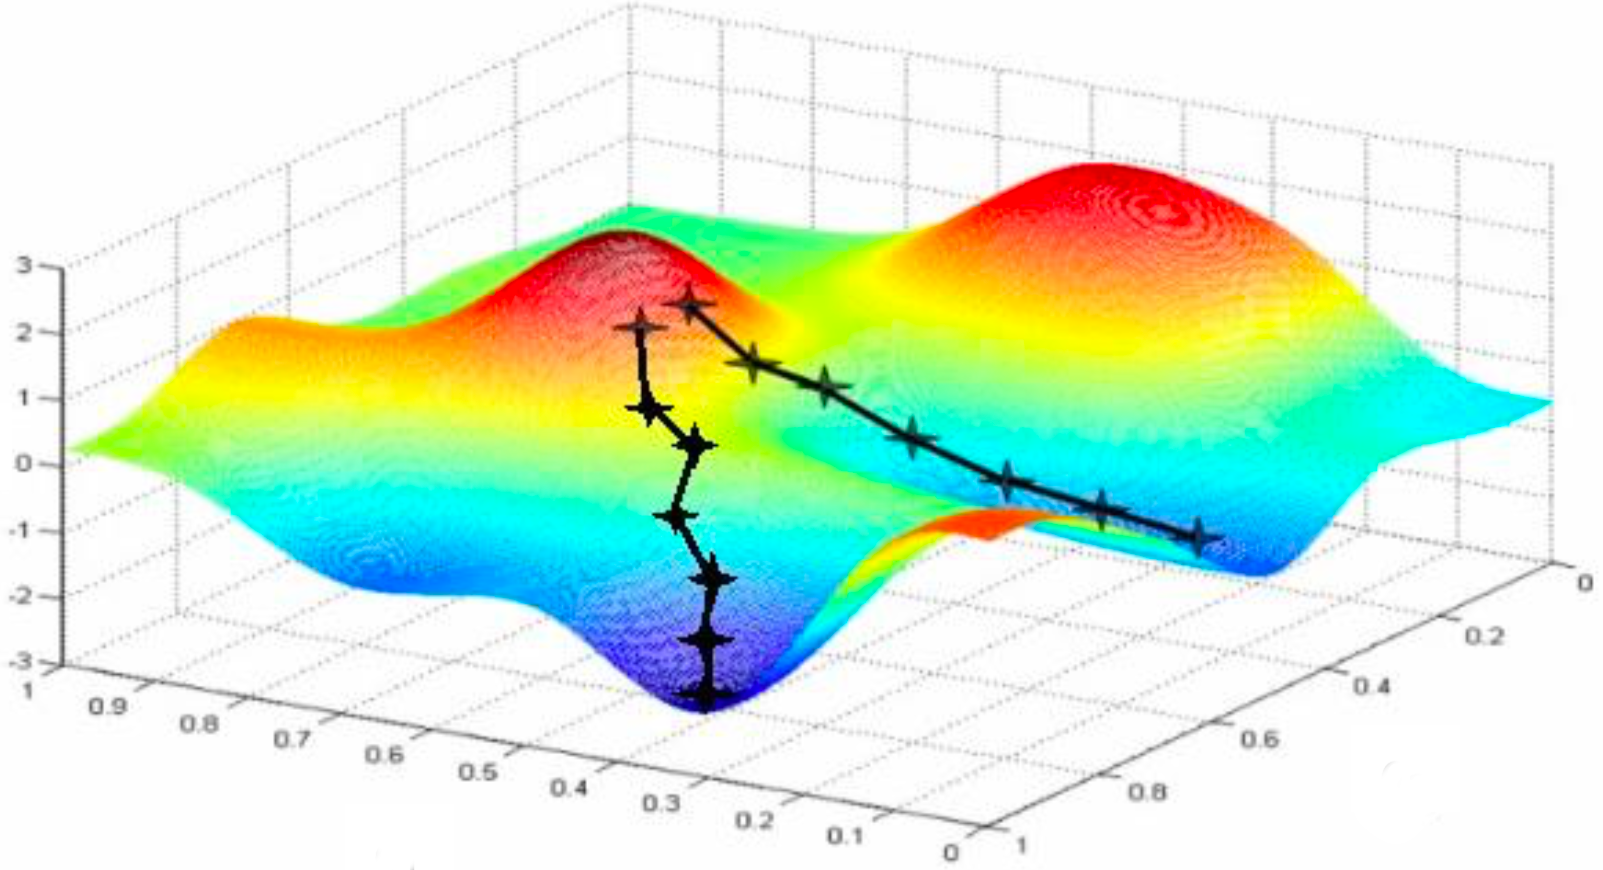
\includegraphics[width=0.5\textwidth]{figs/gdsurface}
\end{frame}


\begin{frame}{gradient descent (GD) is miserable}

\begin{pseudo*}
\pr{gd}(p)\text{:} \\+
    for $s = 1,2,\dots$: \\+
        $p \gets p - \eta \grad C(p)$ \\-
    return $p$
\end{pseudo*}

\vspace{-25mm}
\hfill 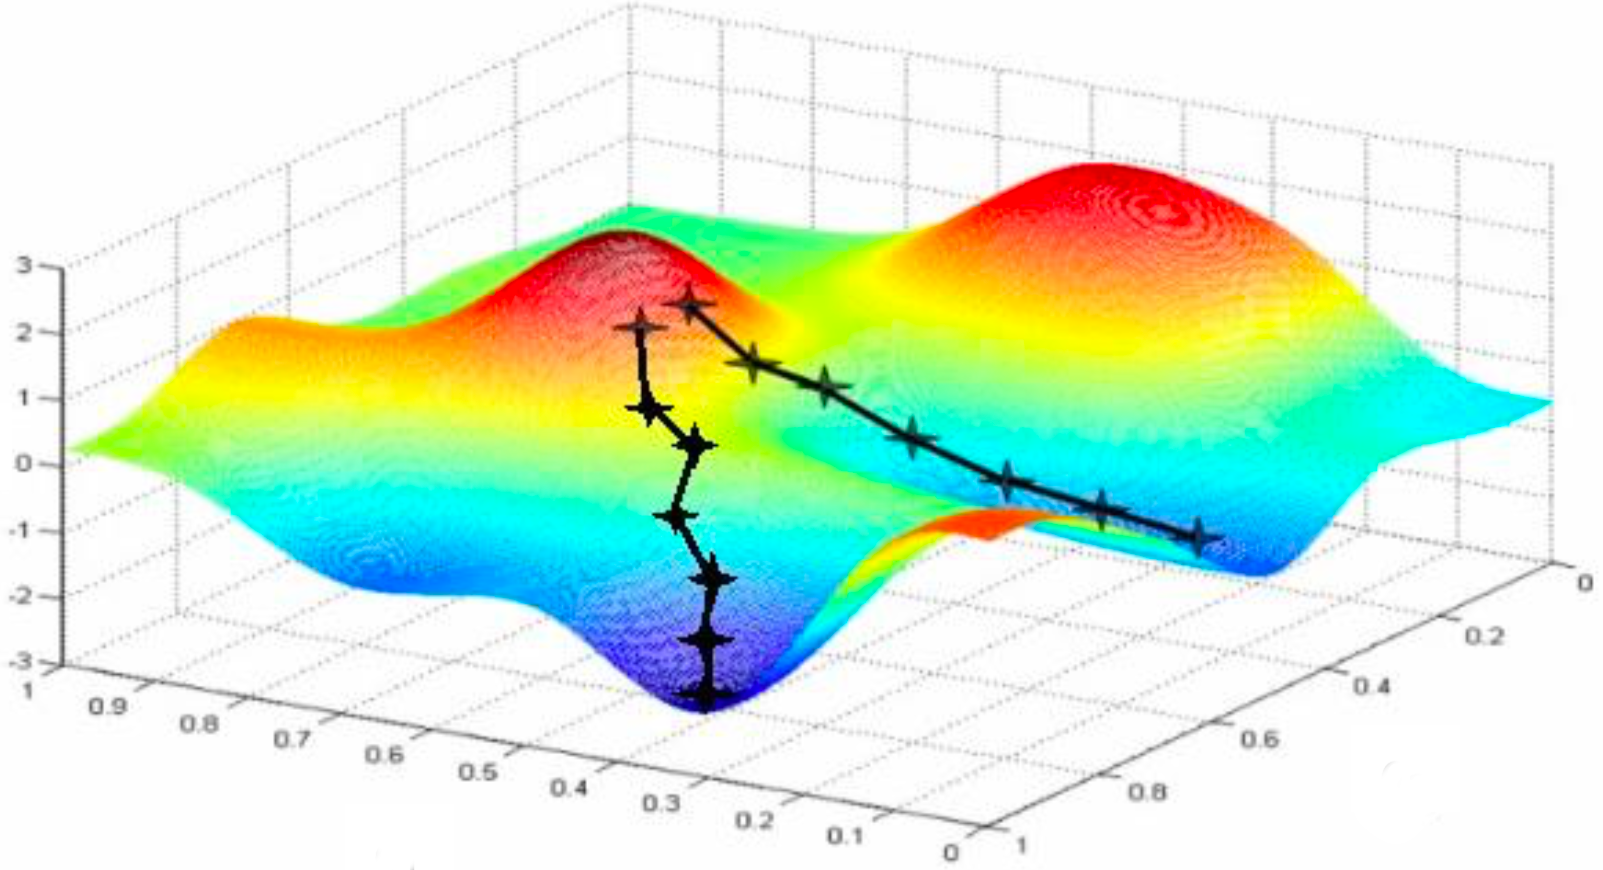
\includegraphics[width=0.35\textwidth]{figs/gdsurface} \phantom{adslj}

\medskip
\begin{itemize}
\item GD is simple to program
    \begin{itemize}
    \item[$\circ$] \dots but it will always let you down
    \end{itemize}
\item known issues with naive GD:
    \begin{itemize}
    \item[$\circ$] it is not clear how far to step \hfill (how to set $\eta$?)
        \begin{itemize}
        \item $C(p)$, $\grad C(p)$ provide no information
        \item provable convergence requires a \emph{line search} or \emph{trust region} approach,  otherwise $G(p)$ may not even decrease
        \item $\eta$ is called the \alert{learning rate} in machine learning
        \end{itemize}
    \item[$\circ$] if GD converges, it may be to a \emph{local} minimum only
    \end{itemize}
\end{itemize}
\end{frame}


\begin{frame}{gradient descent in machine learning: the 2 insights}

\begin{itemize}
\item GD is widely used for training in \alert{machine learning} (ML)
    \begin{itemize}
    \item[$\circ$] a seminar priority?: GD limitations, modifications, alternatives
    \end{itemize}

\medskip
\item ML applies 2 ``insights'' (\emph{habits}?) about how GD should work:
    \begin{enumerate}

\bigskip
    \item \alert{stochastic gradient descent}: since $N$ is big, and because overfitting should be avoided, do \emph{not} compute the whole gradient $\grad C(p)$, but instead a randomly chosen $\grad C^{\{i\}}(p)$
        \begin{itemize}
        \item[$\circ$] i.e.~choose data $(x^{\{i\}},y^{\{i\}})$ and do
            $$p \gets p - \eta \grad C^{\{i\}}(p)$$
        \item[$\circ$] or a choose a \alert{batch}: $p \gets p - \eta \frac{1}{m} \sum_{i=1}^m \grad C^{\{k_i\}}(p)$
        \end{itemize}

\bigskip
    \item \alert{back-propagation}: when computing $\grad C^{\{i\}}(p)$, regard the chain rule as information which can be fed backward through the network
        \begin{itemize}
        \item[$\circ$] back-propagation uses info found in computing forward for $C^{\{i\}}(p)$
        \end{itemize}
    \end{enumerate}
\end{itemize}
\end{frame}


\begin{frame}{stochastic gradient descent (SGD)}

\begin{pseudo*}
\pr{sgd}(p)\text{:} \\+
    for $s = 1,2,\dots$: \\+
        $i=$ (\st{random uniform from} $\{1,\dots,N\}$) \\
        $p \gets p - \eta \grad C^{\{i\}}(p)$ \\-
    return $p$
\end{pseudo*}

\begin{itemize}
\item above is \alert{vanilla} SGD
    \begin{itemize}
    \item[$\circ$] note $i$ is chosen \emph{with} replacement
    \end{itemize}
\item variations:
    \begin{itemize}
    \item[$\circ$] choose $i$ without replacement
    \item[$\circ$] batching: $p \gets p - \eta \frac{1}{m} \sum_{i=1}^m \grad C^{\{k_i\}}(p)$
    \item[$\circ$] \alert{online}: $N$ unknown; data pairs $(x^{\{i\}},y^{\{i\}})$ are provided by a stream
    \end{itemize}
\end{itemize}
\end{frame}


\begin{frame}{observations about the cost gradient}

\begin{itemize}
\item[] \qquad \small $\displaystyle C(p) = \frac{1}{N} \sum_{i=1}^N C^{\{i\}}(p), \qquad C^{\{i\}}(p) = \frac{1}{2} \left\|y^{\{i\}} - a^{[L]}\right\|_2^2$ \normalsize

\medskip
\item $N$ = amount of training data\, $\therefore$\, $N$ is (should be) large
\item gradient for one data pair:
\begin{align*}
\grad C^{\{i\}}(p) &= \grad\left[\frac{1}{2} (y^{\{i\}} - a^{[L]})^\top (y^{\{i\}} - a^{[L]})\right] \\
    &= - \sum_{j=1}^{n_L} (y_j^{\{i\}} - a^{[L]}_j)\, \grad a^{[L]}_j
\end{align*}
\item chain rule will be needed to expand further
    \begin{itemize}
    \item[$\circ$] network output $a_j^{[L]}$ is a \emph{composition} of matrix-vector products and (nonlinear) $\sigma$ applications
    \end{itemize}
\item how to compute $\grad a^{[L]}_j$ efficiently? \dots time for the chain rule!
\end{itemize}
\end{frame}


\begin{frame}{interlude: the buzzword list}

\begin{itemize}
\item \alert{artificial neuron}
    \begin{itemize}
    \item[$\circ$] \alert{activation}
    \item[$\circ$] \alert{activation function}
        \begin{itemize}
        \item sigmoid, ReLU
        \end{itemize}
    \item[$\circ$] \alert{weight} matrix
    \item[$\circ$] \alert{bias} vector
    \end{itemize}
\item \alert{artificial neural network} = ANN
    \begin{itemize}
    \item[$\circ$] feed-forward network
    \end{itemize}
\item \alert{training}
    \begin{itemize}
    \item[$\circ$] \alert{supervised learning}
    \item[$\circ$] labeled data
    \item[$\circ$] nonlinear least-squares optimization
    \end{itemize}
\item \alert{stochastic gradient descent} $=$ SGD
    \begin{itemize}
    \item[$\circ$] learning rate
    \end{itemize}
\item \alert{back-propagation} $=$ BP

\hspace{-7mm} \hrulefill
\item \alert{machine learning} $=$ ML
    \begin{itemize}
    \item[$\circ$] \alert{deep learning} if $L>2$
    \end{itemize}
\end{itemize}
\end{frame}


\section{backward through a neural net}

\begin{frame}{Outline}
  \tableofcontents[hideallsubsections,currentsection]
\end{frame}


\begin{frame}{cost gradient with respect to weights and biases}

\begin{itemize}
\item recall:
    \begin{itemize}
    \item[$\circ$] $p = \{W^{[2]},W^{[3]},\dots,W^{[L]},b^{[2]},b^{[3]},\dots,b^{[L]}\} \in \RR^s$ is a grab-bag of parameters
    \item[$\circ$] cost for one pair $(x^{\{i\}},y^{\{i\}})$:  \qquad \small $\displaystyle C^{\{i\}}(p) = \frac{1}{2} \left\|y^{\{i\}} - a^{[L]}\right\|_2^2$ \normalsize
    \end{itemize}

\medskip
\item want: \qquad \small  $\displaystyle \grad C^{\{i\}}(p) = \left[\frac{\partial C^{\{i\}}}{\partial p_1},\dots,\frac{\partial C^{\{i\}}}{\partial p_s}\right]$ \normalsize
\item the components of this gradient come in two types:
    $$\frac{\partial C^{\{i\}}}{\partial w_{jk}^{[\ell]}}, \quad \frac{\partial C^{\{i\}}}{\partial b_j^{[\ell]}}$$
\end{itemize}
\end{frame}


\begin{frame}{chain rule on the cost (for the last layer)}

\begin{itemize}
\item recall:\quad $\displaystyle z_j^{[L]} = \sum_{k=1}^{n_{L-1}} w_{jk}^{[L]} a_k^{[L-1]} + b_j^{[L]}$
\item expand the 2-norm and the activation in the one-pair cost formula:
    $$C^{\{i\}}(p) = \frac{1}{2} \sum_{j=1}^{n_L} (y_j^{\{i\}} - \underbrace{\sigma(z_j^{[L]})}_{= a_j^{[L]}})^2$$

\vspace{-4mm}
\item thus by the chain rule:
\begin{align*}
\frac{\partial C^{\{i\}}}{\partial w_{jk}^{[L]}} &= \boxed{\frac{\partial C^{\{i\}}}{\partial z_j^{[L]}}}\, \frac{\partial z_j^{[L]}}{\partial w_{jk}^{[L]}} = \boxed{\frac{\partial C^{\{i\}}}{\partial z_j^{[L]}}}\, a_k^{[L-1]} \\
\frac{\partial C^{\{i\}}}{\partial b_{j}^{[L]}} &= \boxed{\frac{\partial C^{\{i\}}}{\partial z_j^{[L]}}}\, \frac{\partial z_j^{[L]}}{\partial b_{j}^{[L]}} = \boxed{\frac{\partial C^{\{i\}}}{\partial z_j^{[L]}}}
\end{align*}
    \begin{itemize}
    \item[$\circ$] the boxed quantity shows up a lot, so it gets a name \dots
    \end{itemize}
\end{itemize}
\end{frame}


\begin{frame}{chain rule on the cost}

\begin{itemize}
\item define, following HH19:
    $$\delta_j^{[\ell]} = \frac{\partial C^{\{i\}}}{\partial z_j^{[\ell]}}$$

    \begin{itemize}
    \item[$\circ$] this definition is for \emph{any layer} $\ell$
    \item[$\circ$] remember that this is for one data pair $(x^{\{i\}},y^{\{i\}})$
    \end{itemize}
\item for the final layer $\ell=L$ we already have:
\begin{align*}
\delta_j^{[L]} &= - (y_j^{\{i\}} - a_j^{[L]})\, \sigma'(z_j^{[L]}) \\
\frac{\partial C^{\{i\}}}{\partial w_{jk}^{[L]}} &= \delta_j^{[L]} a_k^{[L-1]} \\
\frac{\partial C^{\{i\}}}{\partial b_{j}^{[L]}} &= \delta_j^{[L]}
\end{align*}
\end{itemize}
\end{frame}


\begin{frame}{chain rule on the cost}

\begin{itemize}
\item to go further back into the network, follow multiple routes:
\begin{quote}
$a_j^{[L]}$ depends on $a_k^{[L-1]}$ for different $k$, then $a_k^{[L-1]}$ depends on $a_s^{[L-2]}$ for different $s$, \dots
\end{quote}
\item example: \quad what is derivative of cost $C^{\{i\}}$ with respect to \small ${\color{red} w_{43}^{[3]}}$\normalsize?

\begin{center}
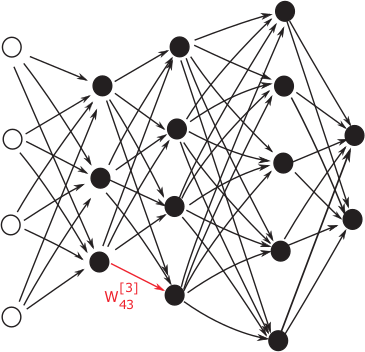
\includegraphics[width=0.4\textwidth]{figs/bigredw}
\end{center}
\end{itemize}
\end{frame}


\begin{frame}{find inside the chain rule: multiplication by the transpose}

\begin{itemize}
\item \emph{example.} $L=4$; consider a weight into layer $\ell=3$:
   $$\frac{\partial C^{\{i\}}}{\partial w_{jk}^{[3]}} = \underbrace{\frac{\partial C^{\{i\}}}{\partial z_{j}^{[3]}}}_{multi-route} \underbrace{\frac{\partial z_{j}^{[3]}}{\partial w_{jk}^{[3]}}}_{easy} = \delta_j^{[3]} a_{k}^{[2]} \phantom{sdlkjaf ajdsf lkadfj sdafkj}$$

\vspace{-25mm}
\hfill 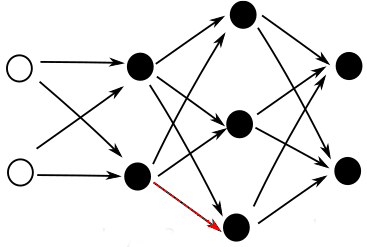
\includegraphics[width=0.3\textwidth]{figs/redcleannet}
\item but $\delta_j^{[3]}$ relates to the \emph{next}-layer deltas $\delta^{[4]}$ by matrix multiplication:
\begin{align*}
\delta_j^{[3]} = \frac{\partial C^{\{i\}}}{\partial z_{j}^{[3]}} &= \sum_{s=1}^{n_4} \frac{\partial C^{\{i\}}}{\partial z_{s}^{[4]}} \frac{\partial z_{s}^{[4]}}{\partial z_{j}^{[3]}} \\
  &= \sum_{s=1}^{n_4} \delta_s^{[4]} \frac{\partial z_{s}^{[4]}}{\partial a_{j}^{[3]}} \frac{\partial a_{j}^{[3]}}{\partial z_{j}^{[3]}} \\
  &= \sum_{s=1}^{n_4} \delta_s^{[4]} w_{sj}^{[4]} \sigma'(z_{j}^{[3]}) = \left((W^{[4]})^\top \delta^{[4]}\right)_j \sigma'(z_{j}^{[3]})
\end{align*}
\end{itemize}
\end{frame}


\begin{frame}{the heart of back-propagation}

\begin{itemize}
\item define the entrywise (\emph{Hadamard}?) product of vectors $x,y\in\RR^m$:
    $$(x\circ y)_j = x_j y_j$$

\begin{lemma}
the vector $\displaystyle \delta^{[\ell]} = \left[\frac{\partial C^{\{i\}}}{\partial z_j^{[\ell]}}\right]  \in \RR^{n_{\ell}}$ can be computed by (back-) multiplying the weight matrix transposes (adjoints):
\begin{align*}
\delta^{[L]} &= \sigma'(z^{[L]}) \circ (a^{[L]} - y^{\{i\}}), \\
\delta^{[\ell]} &= \sigma'(z^{[\ell]}) \circ \underbrace{(W^{[\ell+1]})^\top \delta^{[\ell+1]}}_{\text{matrix-vector product}}, \qquad \ell = L-1,L-2,\dots,2
\end{align*}
\end{lemma}

\bigskip
\item \emph{key point:} start with last layer $\ell=L$ and count \emph{down} to $\ell=2$
\end{itemize}
\end{frame}


\begin{frame}{back-propagation provides the cost gradient}

\begin{corollary}
once the $\delta^{[\ell]}$ are calculated, all components of the gradient are easy:
\begin{align*}
\frac{\partial C^{\{i\}}}{\partial w_{jk}^{[\ell]}} &= \delta_j^{[\ell]} a_k^{[\ell-1]}, \qquad \frac{\partial C^{\{i\}}}{\partial b_{j}^{[\ell]}} = \delta_j^{[\ell]}
\end{align*}
for $\ell = 2,\dots,L$
\end{corollary}

\bigskip
\begin{itemize}
\item \emph{observation:}  the derivative matrix, with respect to $W^{[\ell]}$, is a rank-one outer product:
    $$\frac{\partial C^{\{i\}}}{\partial W^{[\ell]}} = \delta^{[\ell]} \left(a^{[\ell-1]}\right)^\top$$

\end{itemize}
\end{frame}


\begin{frame}{pseudocode: forward pass with back-propagation}

from $x,y$ and $p=\{W^{[\ell]},b^{[\ell]}\}$ compute $C(p)$ and $\grad C(p)$:

\vspace{-2mm}
\begin{pseudo*}
\pr{forwardbackward}(x,y,W^{[\ell]},b^{[\ell]})\text{:} \\+
    $a^{[1]} = x$ \\
    for $\ell = 2,\dots,L$: \\+
        $z^{[\ell]} = W^{[\ell]} a^{[\ell-1]} + b^{[\ell]}$ \\
        $a^{[\ell]} = \sigma(z^{[\ell]})$, \quad $r^{[\ell]} = \sigma'(z^{[\ell]})$ \\-
    $C = \frac{1}{2} \|y - a^{[L]}\|_2^2$ {\Large \strut} \\
    $\delta^{[L]} = r^{[L]} \circ (a^{[L]} - y)$ {\Large \strut} \\
    for $\ell = L,\dots,2$: \\+
        if $\ell<L$: \\+
            $\delta^{[\ell]} = r^{[\ell]} \circ (W^{[\ell+1]})^\top \delta^{[\ell+1]}$ \\-
        $\frac{\partial C}{\partial W^{[\ell]}} = \delta^{[\ell]} (a^{[\ell-1]})^\top$ {\Large \strut}\\
        $\frac{\partial C}{\partial b^{[\ell]}} = \delta^{[\ell]}$ {\Large \strut} \\-
    return $C,\left\{\frac{\partial C}{\partial W^{[\ell]}}\right\},\left\{\frac{\partial C}{\partial b^{[\ell]}}\right\}$
\end{pseudo*}
\end{frame}


\begin{frame}{pseudocode: training using SGD and BP}

we can integrate SGD into the BP loop (page 873 in HH19):

\vspace{-2mm}
\begin{pseudo*}
\pr{training}(\{x^{\{i\}}\},\{y^{\{i\}}\},\{W^{[\ell]}\},\{b^{[\ell]}\})\text{:} \\+
    for $s = 1,2,\dots$ \\+
        $i=$ (\st{random uniform from} $\{1,\dots,N\}$) \\
	    $a^{[1]} = x^{\{i\}}$ \\
	    for $\ell = 2,\dots,L$: \\+
	        $z^{[\ell]} = W^{[\ell]} a^{[\ell-1]} + b^{[\ell]}$ \\
	        $a^{[\ell]} = \sigma(z^{[\ell]})$, \quad $r^{[\ell]} = \sigma'(z^{[\ell]})$ \\-
	    $\delta^{[L]} = r^{[L]} \circ (a^{[L]} - y^{\{i\}})$ {\Large \strut} \\
	    for $\ell = L,\dots,2$: \\+
	        if $\ell<L$: \\+
	             $\delta^{[\ell]} = r^{[\ell]} \circ (W^{[\ell+1]})^\top \delta^{[\ell+1]}$ \\-
	        $W^{[\ell]} \gets W^{[\ell]} - \eta\, \delta^{[\ell]} (a^{[\ell-1]})^\top$ {\Large \strut}\\
	        $b^{[\ell]} \gets b^{[\ell]} - \eta\, \delta^{[\ell]}$ {\Large \strut} \\--
    return $\{W^{[\ell]}\},\{b^{[\ell]}\}$
\end{pseudo*}
\end{frame}

\section{running the codes yourself}

\begin{frame}{Outline}
  \tableofcontents[hideallsubsections,currentsection]
\end{frame}


\begin{frame}{\emph{Matlab online} instructions: HH19 codes}

\begin{itemize}
\item as a UAF person you have access to Matlab online if you want it

\begin{center}
\href{https://matlab.mathworks.com/}{\texttt{matlab.mathworks.com}}
\end{center}

    \begin{itemize}
    \item[$\circ$] I also use Octave
    \end{itemize}
\item 
\item beamer
\end{itemize}
\end{frame}


\begin{frame}{\emph{Matlab online} instructions: my versions of HH19 codes}

\begin{itemize}
\item FIXME
\item beamer
\end{itemize}
\end{frame}


\section{things that bother me}

\begin{frame}{Outline}
  \tableofcontents[hideallsubsections,currentsection]
\end{frame}


\begin{frame}{fixme}

\begin{itemize}
\item latex
\item beamer
\end{itemize}
\end{frame}


\begin{frame}{future topics?}

\begin{itemize}
\item CNN
\item GNN
\item Newton and Quasi-Newton optimization methods
    \begin{itemize}
    \item[$\circ$] L-BFGS
    \end{itemize}
\item stochastic optimization
    \begin{itemize}
    \item[$\circ$] online machine learning
    \item[$\circ$] Adam
    \end{itemize}
\end{itemize}
\end{frame}

\end{document}
